\documentclass[12pt, twoside]{article}
\usepackage[letterpaper, margin=1in, headsep=0.5in]{geometry}
\usepackage[english]{babel}
\usepackage[utf8]{inputenc}
\usepackage{amsmath}
\usepackage{amsfonts}
\usepackage{amssymb}
\usepackage{tikz}
\usepackage{venndiagram}
\usetikzlibrary{angles, quotes, arrows}

\usepackage{graphicx}
\usepackage{enumitem}
\usepackage{multicol}

\usepackage{fancyhdr}
\pagestyle{fancy}
\fancyhf{}
\renewcommand{\headrulewidth}{0pt} % disable the underline of the header

\fancyhead[LE]{\thepage}
\fancyhead[RO]{\thepage \\ Name: \hspace{4cm} \,\\}
\fancyhead[LO]{BECA / Mr. Nortonsmith / IB Mathematics\\* Vector Test\\* 17 January 2020}

\begin{document}
\begin{enumerate}[itemsep=6cm]

    \item Find a value for $n$ that will give vector $\vec{a}$ a magnitude of 7:
    
    \begin{center}
        \item $\vec{a} = \begin{pmatrix} -3 \\ 2 \\ n \end{pmatrix}$
    \end{center}

    \item Find values for $b_x$, $b_y$, and $b_z$ that will make $\vec{b}$ perpendicular to $\vec{a}$ regardless of the value of $m$ in $\vec{a}$:
    
    \begin{center}
        $\vec{a} = \begin{pmatrix} -2 \\ 1 \\ m \end{pmatrix}$ \hspace{2cm}
        $\vec{b} = \begin{pmatrix} b_x \\ b_y \\ b_z \end{pmatrix}$
    \end{center}
        
    \newpage

    \item Let $\vec{a} = \begin{pmatrix} 1 \\ 3 \end{pmatrix}$:

    \vspace{1cm}
        
    \begin{enumerate}[itemsep=4cm]
        \item Find the unit vector for $\vec{a}$:

        \item Consider some vector $\vec{b} = k\vec{a}$ for some positive value of $k$ (that is, $\vec{b}$ is parallel to $\vec{a}$). What is the unit vector of $\vec{b}$:

        \item Consider some vector $\vec{b}$ which is perpendicular to $\vec{a}$. Find a possible value for the unit vector of $\vec{b}$:
        
    \end{enumerate}
    
    \newpage

    \item Consider the path formed by the 4 vectors in the diagram below:

    \vspace{1cm}
    
    \begin{center}
    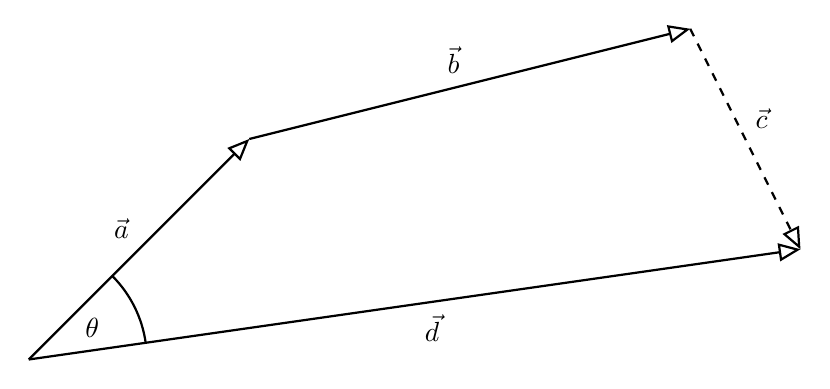
\begin{tikzpicture}[scale=1.4,>=open triangle 45]
        %grid
        \draw[->, thick](0, 0) -- (2, 2) node[midway, above left]{$\vec{a}$};
        \draw[->, thick](2, 2) -- (6, 3) node[midway, above left]{$\vec{b}$};
        \draw[->, thick, dashed](6, 3) -- (7, 1) node[midway, above right]{$\vec{c}$};
        \draw[->, thick](0, 0) -- (7, 1) node[midway, below right]{$\vec{d}$};

        \coordinate (A) at (2,2);
        \coordinate (B) at (0,0);
        \coordinate (C) at (7,1);
        \draw [-, thick] pic [draw=black, angle radius=15mm, "$\theta$"] {angle = C--B--A};
    \end{tikzpicture}
    \end{center}

    \begin{enumerate}
        \vspace{1cm}

        \item Write an equation for $\vec{c}$ in terms of $\vec{a}$, $\vec{b}$, and $\vec{d}$:
        
        \vspace{3cm}
        
        \item Given the following values for $\vec{a}$, $\vec{b}$, and $\vec{d}$, calculate the value of $\vec{c}$:
        
        \vspace{1cm}
        
        \begin{center}
        $\vec{a} = \begin{pmatrix} 2 \\ 2 \end{pmatrix}$ \hspace{1.5cm}
        $\vec{b} = \begin{pmatrix} 4 \\ 1 \end{pmatrix}$ \hspace{1.5cm}
        $\vec{d} = \begin{pmatrix} 7 \\ 1 \end{pmatrix}$
        \end{center}
        
        \vspace{3cm}
        
        \item For the above values vector values, calculate the angle $\theta$ between the $\vec{a}$ and $\vec{d}$:
        
    \end{enumerate}
    
    \newpage

    \item In the diagram below, $\vec{a}$ and $\vec{b}$ are both unit vectors with a $45^\circ$ angle between them. Find the value of the dot product $\vec{a} \cdot \vec{b}$:
    
    \begin{center}
        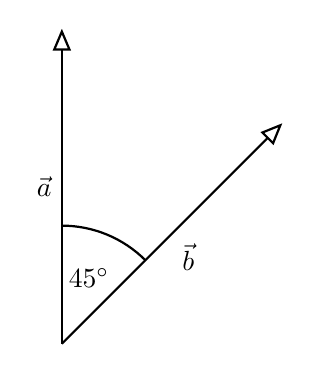
\begin{tikzpicture}[scale=2,>=open triangle 45]
            \draw[->, thick](0, 0) -- (0, 2) node[midway, left]{$\vec{a}$};
            \draw[->, thick](0, 0) -- (1.4, 1.4) node[midway, below right]{$\vec{b}$};

            \coordinate (A) at (0,2);
            \coordinate (B) at (0,0);
            \coordinate (C) at (2,2);

            \draw [-, thick] pic [draw=black, angle radius=15mm, "$45^\circ$"] {angle = C--B--A};
        \end{tikzpicture}
    \end{center}
    
    \newpage
    
    \item Mark each of the following statements as either True or False:
    
    \begin{enumerate}[itemsep=1cm]
        \item For a given vector $\vec{a}$, there are infinitely many vectors $\vec{b}$ such that $\vec{b}$ is parallel to $\vec{a}$. True or False?
        
        \item For a given vector $\vec{a}$, there are infinitely many \emph{unit} vectors $\vec{b}$ such that $\vec{b}$ is parallel to $\vec{a}$. True or False?
        
        \item If $\vec{a}$ and $\vec{b}$ are perpendicular, then the unit vectors for $\vec{a}$ and $\vec{b}$ are also perpendicular. True or False?
        
        \item If $\vec{a}$ and $\vec{b}$ are parallel and $\vec{a} \cdot \vec{b} = |\vec{a}|^2$ (the magnitude of $\vec{a}$ squared), then $\vec{a}$ must $\vec{b}$ must have the same magnitude. True or False?
        
        \item If the angle between $\vec{a}$ and $\vec{b}$ is $30^\circ$, then the angle between $2\vec{a}$ and $2\vec{b}$ must be $60^\circ$. True or False?
    \end{enumerate}

    \newpage

    \item Challenge Problem (extra credit):
    
    \begin{center}
        \vspace{.5cm}
        Consider the following three vectors: \\
        \vspace{1cm}
        $\vec{a} = \begin{pmatrix} 1 \\ 2 \\ -3 \end{pmatrix}$ \hspace{1.5cm}
        $\vec{b} = \begin{pmatrix} 5 \\ -1 \\ 1 \end{pmatrix}$ \hspace{1.5cm}
        $\vec{c} = \begin{pmatrix} 1 \\ c_y \\ c_z \end{pmatrix}$
    \end{center}

    \vspace{.5cm}
    
    Find the values for $c_y$ and $c_z$ that make $\vec{c}$ perpendicular to both $\vec{a}$ and $\vec{b}$ at the same time: (\emph{hint: start by setting up the dot-product equations})
    
\end{enumerate}
\end{document}
